\subsection{Software}
Im folgenden wird die Ansteuerung und Auswertung der elektrischen Komponenten näher beschrieben. Außerdem wird die Kommunikation zwischen der Host- und Target-Plattform erläutert. Als Zielplattform wird ein \ac{BBB} verwendet, auf welchem eine Linux-Distribution ausgeführt wird. In der folgenden Abbildung sind die einzelnen Bausteine und deren Verbindung zu der Zielplattform dargestellt.

\begin{figure}[!h]
\centering
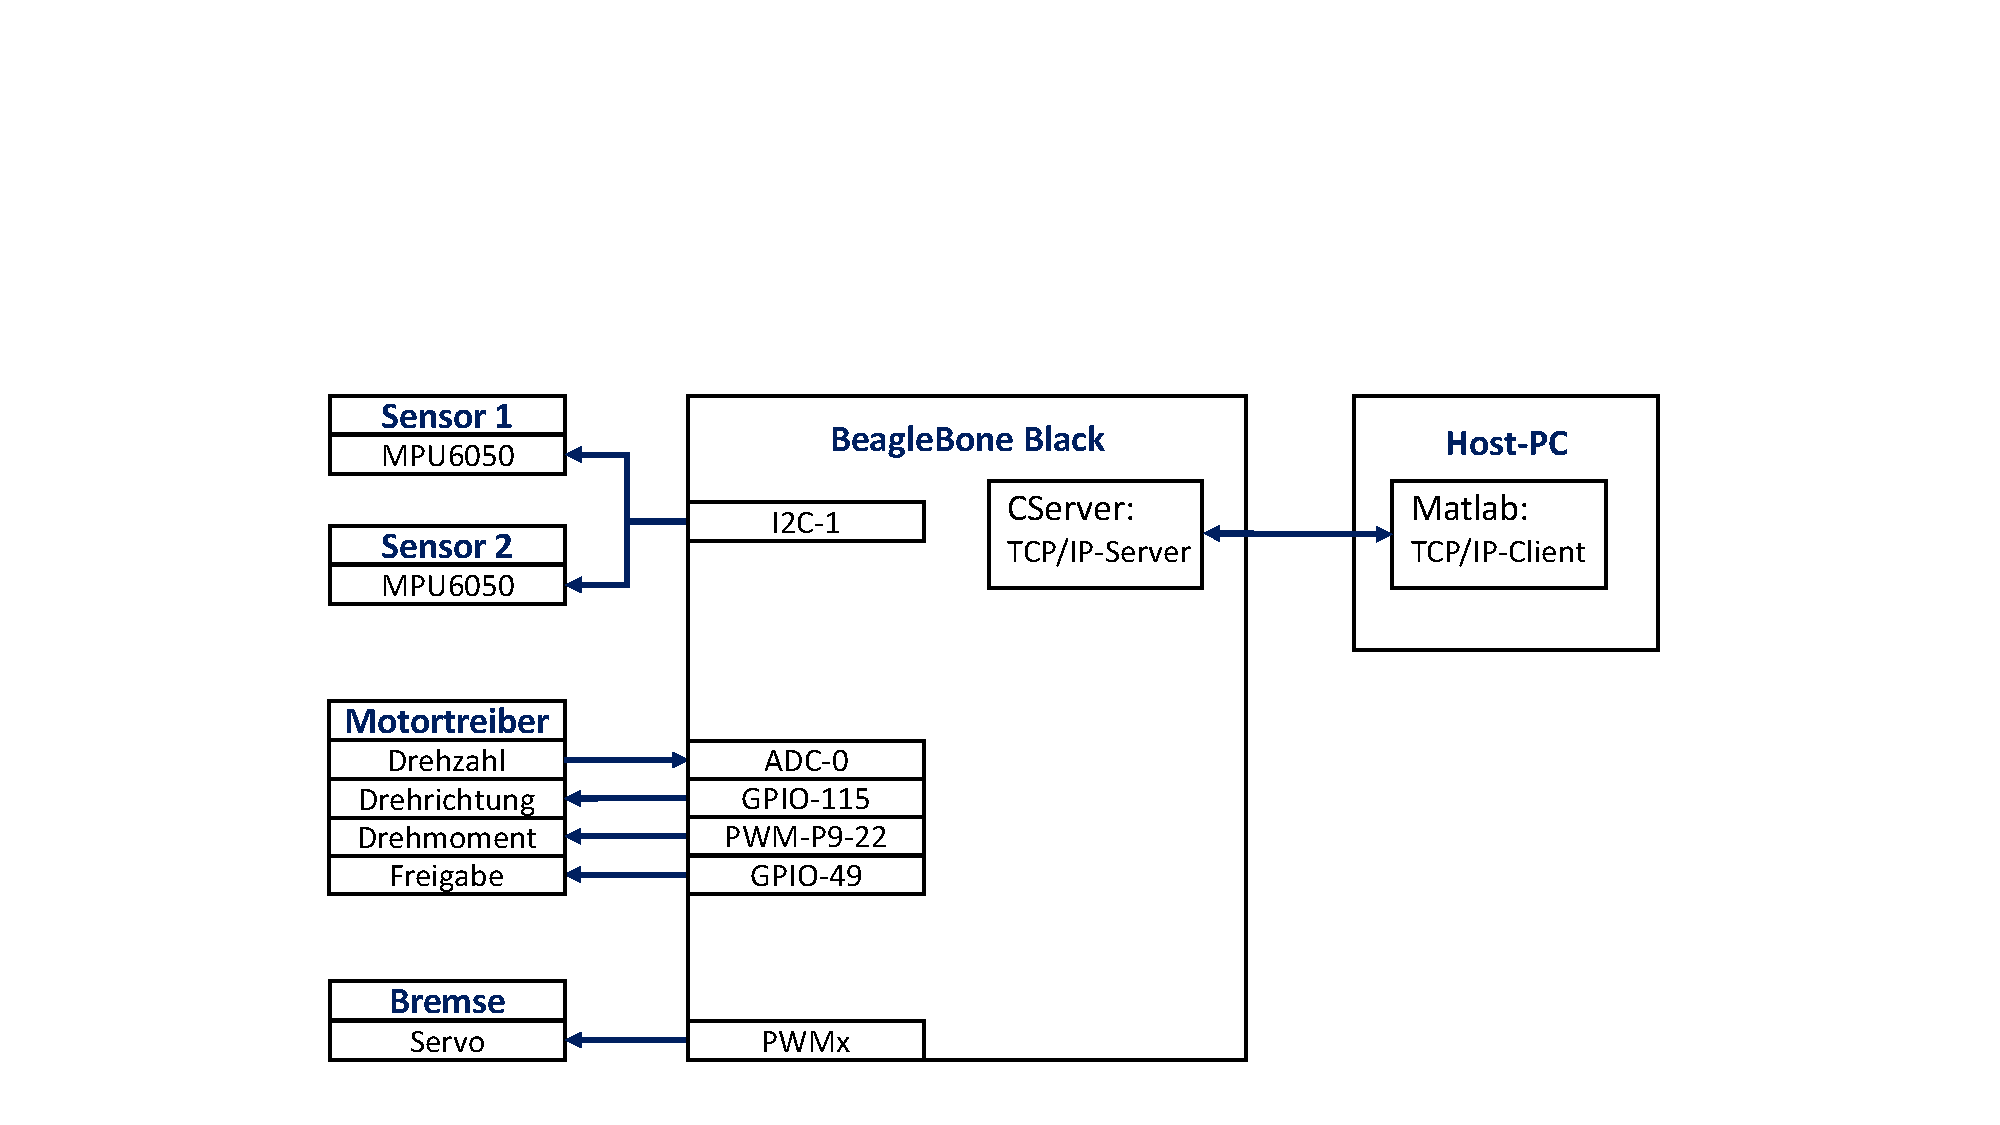
\includegraphics[width=0.8\linewidth, trim={4cm 1cm 5cm 6cm},clip]{img/ElekAufbau_Kommunikation}
\caption{Blockschaltbild der Komponenten, Quelle: eigene Darstellung}
\end{figure}

Um die verschiedenen Versuche und Messungen durchzuführen wird eine Software-Basis entworfen, welche als Grundlage für die verschiedenen Applikationen dient. Diese Grundlage umfasst eine objektorientierte Kapselung der Hardware, die TCP-Server-Implementierung um mit der MATLAB-Anwendung zu kommunizieren, die Definition zweier Komponenten, welche als separate Tasks ausgeführt werden und eine Kommunikationsstruktur für den Datenaustausch. Der Aufbau dieser Bausteine wird in den folgenden Abschnitten näher erläutert. Insgesamt werden acht Versuche durchgeführt:

\begin{itemize}
 \item V1: Bestimmung eines Ausgleichspolynoms um die Sensorwerte in SI-Einheiten umzurechnen. Hierfür werden die X- und Y-Beschleunigungswerte der beiden Sensoren benötigt.
 \item V2: Bestimmung des Offset der Gyroscopes. Hierfür werden die Z-Winkelgeschwindigkeiten der beiden Sensoren benötigt.
 \item V3: Bestimmung eines Ausgleichspolynoms um die ADC-Werte in SI-Einheiten umzurechnen. Hierfür werden die ADC-Werte der Motorgeschwindigkeit benötigt.
 \item V4: Test der Filter für $\varphi$, $\dot{\varphi}$ und ($\psi$). Hierfür müssen die verschiedenen Filter in SW realisiert werden.
 \item V5: Bestimmung des Reibwertes $C_{\varphi}$.
 \item V6: Bestimmung des Rebiwertes $C_{\psi}$.
 \item V7: Test und Bewertung des Regelkreises. Hierfür muss der Regelalgorithmus in SW realisiert werden.
 \item V8: Auspringen...
\end{itemize}

\subsubsection{Hardware-Schnittstelle}
Die Interaktion mit den Treibern des Betriebssystems wird mit Hilfe von Klassen gekapselt. Dadurch entsteht eine einheitliche und benutzerfreundliche Schnittstelle zwischen Hard- und Software. Die Klasse zur Interaktion mit der Hardware muss das folgende Interface erfüllen.

\newpage
\begin{lstlisting}
class IHardware
{
public:
	virtual Int16 getX1__dd_raw() = 0;
	virtual Int16 getX2__dd_raw() = 0;
	virtual Int16 getY1__dd_raw() = 0;
	virtual Int16 getY2__dd_raw() = 0;
	virtual Int16 getPhi1__d_raw() = 0;
	virtual Int16 getPhi2__d_raw() = 0;
	virtual UInt16 getPsi__d_raw() = 0;
	virtual void openBrake() = 0;
	virtual void closeBrake() = 0;
	virtual void enableMotor() = 0;
	virtual void disableMotor() = 0;
	virtual void setTorque(const Float32 torque) = 0;
public:
	IHardware() = default;
	IHardware(const IHardware&) = delete;
	IHardware& operator=(const IHardware&) = delete;
	virtual ~IHardware() = default;
};

\end{lstlisting}

\subsubsection{TCP/IP-Verbindung}
Die Kommunikation zwischen der \ac{BBB}- und der MATLAB-Applikation verläuft über eine TCP/IP-Verbindung. Hierfür wird auf dem \ac{BBB} ein Server ausgeführt, welcher auf die Verbindungsanfrage des MATLAB-Clients wartet. Die Vorteile des gewählten Protokolls liegen einerseits in der gesicherten und abstrahierten Datenübertragung, andererseits in den anwendungsfreundlichen Bibliotheken für Linux und MATLAB. Mit Hilfe einer simulierten Ethernet-Verbindung über USB wird ein privates Netzwerk zwischen der Zielplattform und dem Entwiclungs-PC eingerichtet.

Bild mit Adressen/Socket, etc.

\subsubsection{Komponentenarchitektur}
Die Hauptaufgaben der Applikation werden auf zwei Komponenten verteilt. Die erste übernimmt die Auswertung der Sensorik, Berechnung der Filter- und Regelalgorithmen und Ansteuerung der Aktorik. Hierfür werden Klasen eingeführt um die verschiedenen Teilaufgaben getrennt zu bearbeiten und einen übersichtlichen Software-Entwurf zu erhalten. Die Hauptaufgabe der zweiten Komponente besteht in der Kommunikation mit der MATLAB-Applikation, welche mit Hilfe eines TCP/IP-Servers erfolgt. 
Die beiden Komponenten werden von einer abstrakten Basisklasse abgeleitet und in eigenständigen Prozessen ausgeführt. In der Elternklasse werden rein virtuelle Methoden festgehalten welche zur Initialisierung und Durchführung der verschiedenen Versuche dienen. Somit ist es möglich die Grundstruktur für die mehreren Applikationen wiederzuverwenden. Auf Grund der simplen Abläufe genügt ein Flag um wiederzugeben ob sich eine Komponente im \textit{STANDBY}- oder \textit{RUNNING}-Zustand befinden. Für komplexere Anwendung kann an dieser Stelle ein vollständiger Zustandsautomat implementiert werden.

\begin{lstlisting}
class AComponentBase
{
public:
	virtual void init() = 0;
	virtual void run_V1_AusgleichsPolynomAccelerometer() = 0;
	virtual void run_V2_OffsetGyroscope() = 0;
	virtual void run_V3_AusgleichsPolynomMotorADC() = 0;
	virtual void run_V4_FilterTest() = 0;
	virtual void run_V5_BestimmungC_psi() = 0;
	virtual void run_V6_BestimmungC_phi() = 0;
	virtual void run_V7_RegelungTest() = 0;
public:
	AComponentBase(TQueue<Config::QueueSize>& rxQueue,
				   TQueue<Config::QueueSize>& txQueue,
				   bool initStandby);
	AComponentBase() = delete;
	AComponentBase(const AComponentBase&) = delete;
	AComponentBase& operator=(const AComponentBase&) = delete;
	virtual ~AComponentBase() = default;
protected:
	TQueue<Config::QueueSize>& mRxQueue;
	TQueue<Config::QueueSize>& mTxQueue;
	bool mStandbyState;
	UInt8 mPadding{};
};

\end{lstlisting}

Die Kommunikation der beiden Prozess auf dem \ac{BBB} erfolgt mit Hilfe von Nachrichten. Dieser werden mit Hilfe von Queues, welche im \ac{SHM} angelegt werden, zwischen den beiden Prozessen ausgetauscht. Zusätzlich wird dieselbe Nachrichtenstruktur verwendet um Daten zwischen dem \ac{BBB} und der MATLAB-Anwendung auszutauschen. Hierfür werden die Daten als Byte-Stream über die TCP/IP-Verbindung übertragen. 

\begin{figure}[!h]
\centering
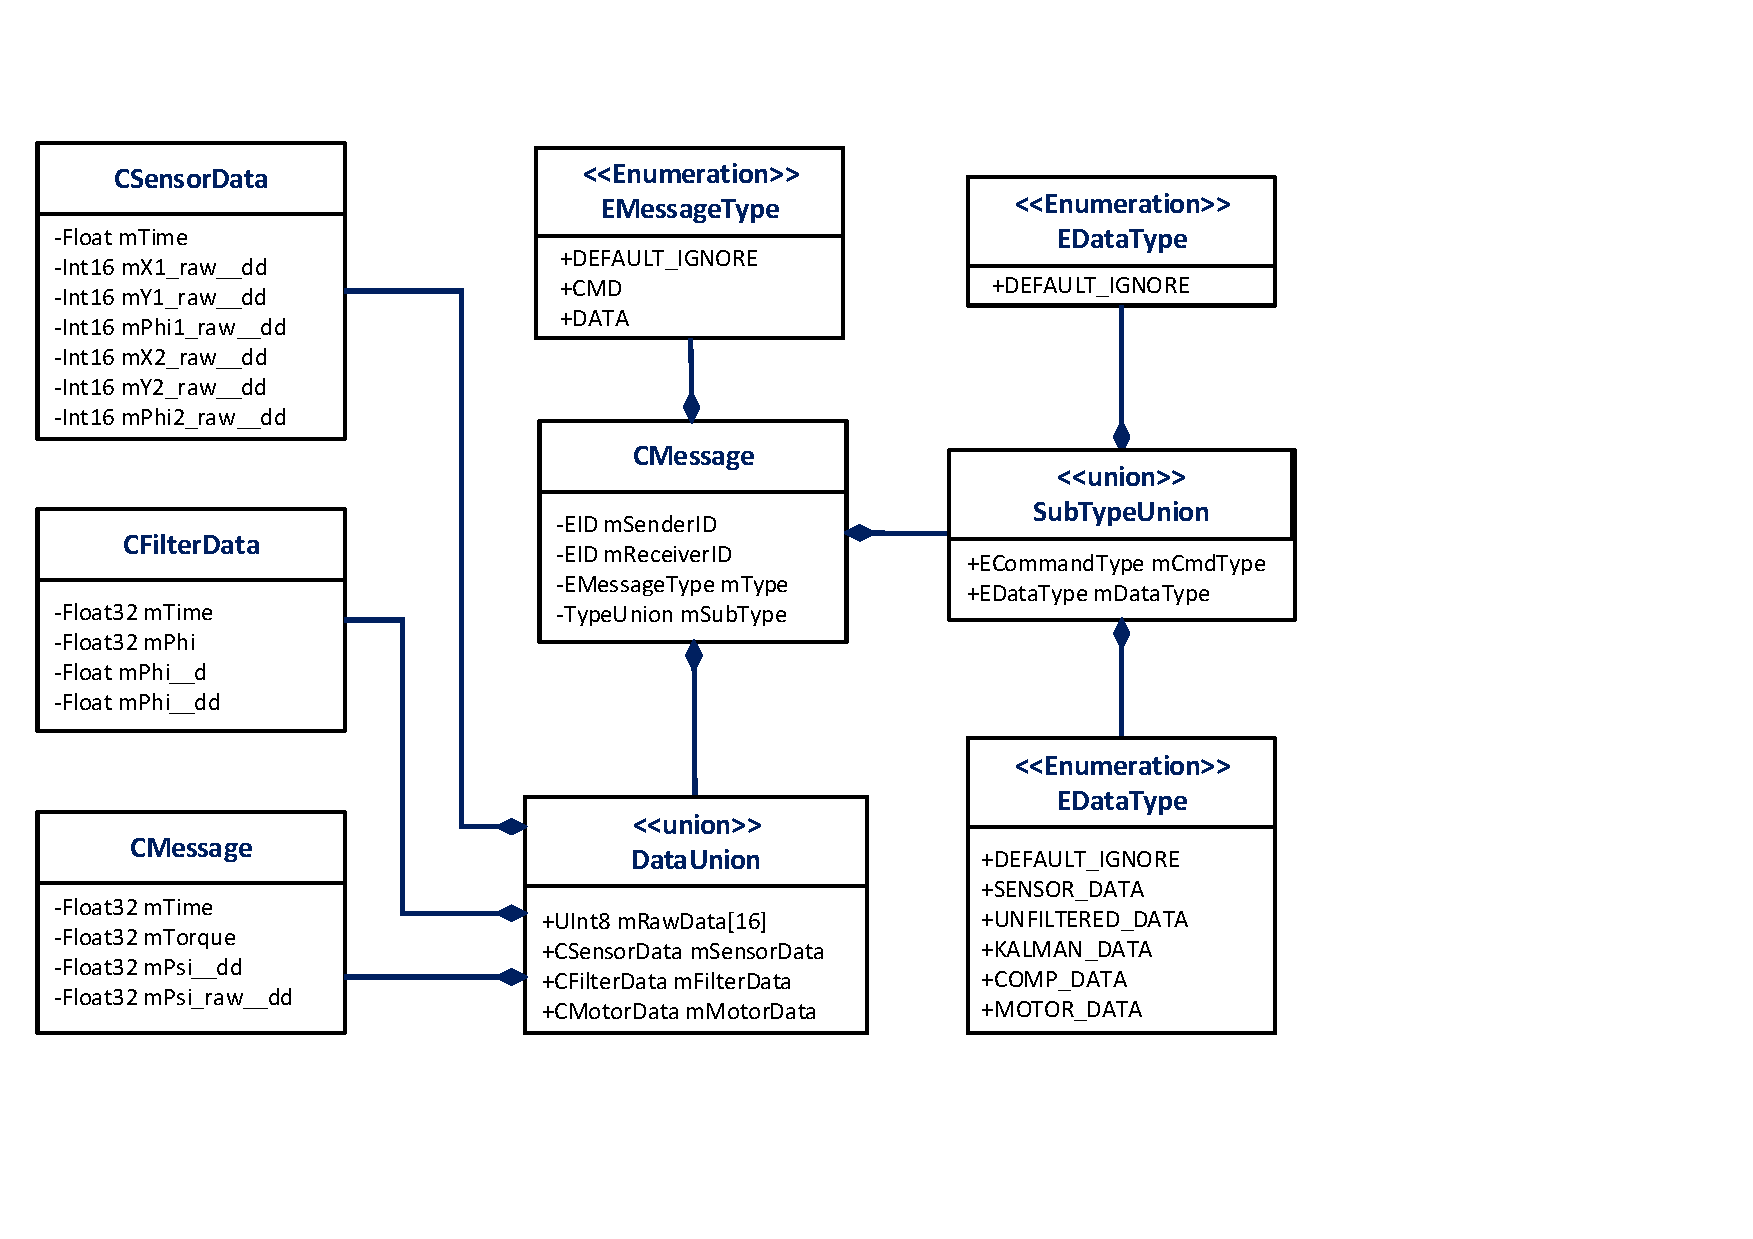
\includegraphics[width=0.8\linewidth, trim={0cm 0cm 7cm 5cm},clip]{img/UML_MessageClassDiag}
\caption{UML Nachrichtenaufbau, Quelle: eigene Darstellung}
\end{figure}

Die Nachrichten bestehen aus einem Header, welcher das Ereignis und weitere Informationen, wie z.B. den Typ der enthaltenen Daten. Das Datenfeld wird genutzt um relevante Informationen wie Sensor-, Filter- und Motorwerte an die MATLAB-Applikation zu übermitteln. Die Nachrichten werden in Form einer Klasse realisiert, welche Konstruktoren enthält um die verschiedenen Datenstrukturen in das Datenfeld zu legen.

\subsubsection{Allgemeiner Ablauf der Versuchsapplikationen}
Die Ablauf der unterschiedlichen Versuche ist auf Seite der SW sehr ähnlich. Die beiden Komponenten starten im \textit{STANDBY}-Zustand. Die Kommunikations-Komponente wartet darauf, dass der MATLAB-Client eine Verbindung aufbaut. Daraufhin wechselt diese in den \textit{RUNNING}-Zustand und sendet eine Nachricht an die \textit{Control}-Komponente, welche darauf ebenfalls in den \textit{RUNNING}-Zustand wechselt.
Im Anschluss wertet die \textit{Control}-Komponente in zyklischen Abständen die Sensoren aus, berechnet ggf. Filter- oder Reglerwerte und sendet diese mit Hilfe von Nachrichten an die Kommunikations-Komponente. Diese leitet empfangene Nachrichten an die MATLAB-Applikation weiter, welche diese virtualisiert und zur weiteren Verarbeitung speichert. 
Sobald die MATLAB-Anwendung die Verbindung abbricht wird eine entsprechende Nachricht an die \textit{Control}-Komponente gesendet. Daraufhin terminieren beide Prozesse selbständig.
